\documentclass[border=1pt]{standalone}
\usepackage{fkmath}
\usepackage{tikz}
\makeatletter
\tikzset{use path/.code=\tikz@addmode{\pgfsyssoftpath@setcurrentpath#1}}
\makeatother
\begin{document}
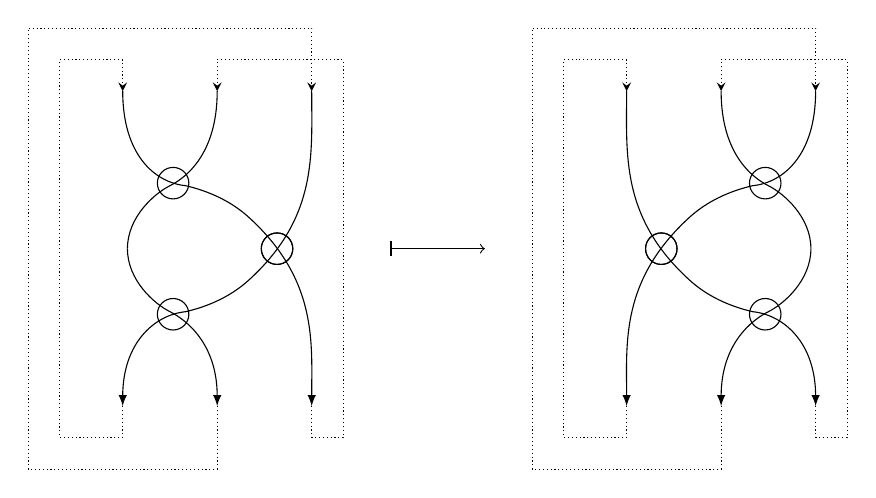
\begin{tikzpicture}[scale=.4, every node/.style={scale=1}]
  \pgfmathsetmacro{\gap}{10pt}

  % \draw[help lines] (-4,-6) grid (4,6);
  \def\pointCols{orange}
  \def\controlPointCols{red}
  \def\theNextPCol{blue}
  \def\theNextCCol{teal}

  \def\defSideReidIII{

    \def\myPointOpacity{0}

    \coordinate (p1) at (-3, 5);
    \coordinate (p2) at (-1, 2);
    \coordinate (p3) at (1, 1);
    \coordinate (p4) at (3,-5);

    % Controls for point 1
    \coordinate (c1a) at (-3, 3);
    \coordinate (c1b) at (-2, 2.1);

    % Controls for point 2
    \coordinate (c2a) at (-.25, 1.825);
    \coordinate (c2b) at (.45, 1.5);

    % Controls for point 3
    \coordinate (c3a) at (3.2, -1);
    \coordinate (c3b) at (3, -3);

    \draw (-1.40, 2.08125)  circle (.5);

    \node[circle, fill opacity=\myPointOpacity, fill=\pointCols, inner sep=.5pt] () at (p1) {};
    \node[circle, fill opacity=\myPointOpacity, fill=\pointCols, inner sep=.5pt] () at (p2) {};
    \node[circle, fill opacity=\myPointOpacity, fill=\pointCols, inner sep=.5pt] () at (p3) {};

    \node[circle, fill opacity=\myPointOpacity, fill=\controlPointCols, inner sep=.5pt] () at (c1a) {};
    \node[circle, fill opacity=\myPointOpacity, fill=\controlPointCols, inner sep=.5pt] () at (c1b) {};
    \node[circle, fill opacity=\myPointOpacity, fill=\controlPointCols, inner sep=.5pt] () at (c2a) {};
    \node[circle, fill opacity=\myPointOpacity, fill=\controlPointCols, inner sep=.5pt] () at (c2b) {};
    \node[circle, fill opacity=\myPointOpacity, fill=\controlPointCols, inner sep=.5pt] () at (c3a) {};
    \node[circle, fill opacity=\myPointOpacity, fill=\controlPointCols, inner sep=.5pt] () at (c3b) {};

    % \path (p1)
    \path[save path=\SideRIII] (p1) .. controls (c1a) and (c1b) .. (p2) .. controls (c2a) and (c2b) .. (p3) .. controls (c3a) and (c3b) .. (p4);
  }

  \def\defMidReidIII{

    \def\myPointOpacity{0}

    \coordinate (p1) at (0, 5);
    \coordinate (p2) at (-1.5, 2);
    \coordinate (p3) at (-2.85, 0);

    % Controls for point 1
    \coordinate (c1a) at (0, 3);
    \coordinate (c1b) at (-1, 2.25);

    % Controls for point 2
    \coordinate (c2a) at (-2, 1.75);
    \coordinate (c2b) at (-2.85, 1);

    % Controls for point 3
    \coordinate (c3a) at (-3, -1);
    \coordinate (c3b) at (-2.5, -1.5);

    \node[circle, fill opacity=\myPointOpacity, fill=\pointCols, inner sep=.5pt] () at (p1) {};
    \node[circle, fill opacity=\myPointOpacity, fill=\pointCols, inner sep=.5pt] () at (p2) {};
    \node[circle, fill opacity=\myPointOpacity, fill=\pointCols, inner sep=.5pt] () at (p3) {};

    \node[circle, fill opacity=\myPointOpacity, fill=\controlPointCols, inner sep=.5pt] () at (c1a) {};
    \node[circle, fill opacity=\myPointOpacity, fill=\controlPointCols, inner sep=.5pt] () at (c1b) {};
    \node[circle, fill opacity=\myPointOpacity, fill=\controlPointCols, inner sep=.5pt] () at (c2a) {};
    \node[circle, fill opacity=\myPointOpacity, fill=\controlPointCols, inner sep=.5pt] () at (c2b) {};
    \node[circle, fill opacity=\myPointOpacity, fill=\controlPointCols, inner sep=.5pt] () at (c3a) {};
    \node[circle, fill opacity=\myPointOpacity, fill=\controlPointCols, inner sep=.5pt] () at (c3b) {};

    \draw (1.9, 0)  circle (.5);

    % \path (p1)
    \path[save path=\MidRIII] (p1) .. controls (c1a) and (c1b) .. (p2) .. controls (c2a) and (c2b) .. (p3);% .. controls (c3a) and (c3b) .. (p4);
  }

  \begin{scope}
    \defSideReidIII
    % \draw[white, line width=7pt, use path=\HalfR];
    \draw[-latex, use path=\SideRIII];

    \defMidReidIII
    % \draw[white, line width=\gap, use path=\MidRIII];
    \draw[use path=\MidRIII];


    \begin{scope}[xscale=1, yscale=-1]
      \defMidReidIII
      % \draw[white, line width=\gap, use path=\MidRIII];
      \draw[latex-, use path=\MidRIII];

      \defSideReidIII
      % \draw[white, line width=\gap, use path=\SideRIII];
      \draw[latex-, use path=\SideRIII];
    \end{scope}

    % \node (i) at (-1.35, 2.85) {$i$};
    % \node (j) at (1.95, 1) {$j$};
    % \node (k) at (-1.35, -1.25) {$k$};

    \draw[-stealth, densely dotted] (3, -5) -- (3, -6) -- (4, -6) -- (4, 6) -- (0, 6) -- (0, 5);
    \draw[-stealth, densely dotted] (0, -5) -- (0, -7) -- (-6, -7) -- (-6, 7) -- (3, 7) -- (3, 5);
    \draw[-stealth, densely dotted] (-3, -5) -- (-3, -6) -- (-5, -6) -- (-5, 6) -- (-3, 6) -- (-3, 5);
  \end{scope}

  \begin{scope}[xshift=16cm]
    \begin{scope}[xscale=-1, yscale=-1]

      \defSideReidIII
      % \draw[white, line width=7pt, use path=\HalfR];
      \draw[latex-, use path=\SideRIII];

      \defMidReidIII
      % \draw[white, line width=\gap, use path=\MidRIII];
      \draw[latex-, use path=\MidRIII];


      \begin{scope}[xscale=1, yscale=-1]
        \defMidReidIII
        % \draw[white, line width=\gap, use path=\MidRIII];
        \draw[use path=\MidRIII];

        \defSideReidIII
        % \draw[white, line width=\gap, use path=\SideRIII];
        \draw[-latex, use path=\SideRIII];
      \end{scope}

      % \node (i) at (-1.45, 1.35) {$i$};
      % \node (j) at (1.8, -1) {$j$};
      % \node (k) at (-1.45, -2.85) {$k$};

    \end{scope}

    \draw[-stealth, densely dotted] (3, -5) -- (3, -6) -- (4, -6) -- (4, 6) -- (0, 6) -- (0, 5);
    \draw[-stealth, densely dotted] (0, -5) -- (0, -7) -- (-6, -7) -- (-6, 7) -- (3, 7) -- (3, 5);
    \draw[-stealth, densely dotted] (-3, -5) -- (-3, -6) -- (-5, -6) -- (-5, 6) -- (-3, 6) -- (-3, 5);

  \end{scope}
  \draw[|->] (5.5,0) -- (8.5,0) node[midway, above] {};
\end{tikzpicture}
\end{document}
